\section{SOFTWARE SPECIFIC PROCESSES \label{sec:software_specific_processes}}

	\subsection{SOFTWARE IMPLEMENTATION PROCESSES\label{subsec:software_implementation_processes}}

		\begin{figure}[h]
			\centering
			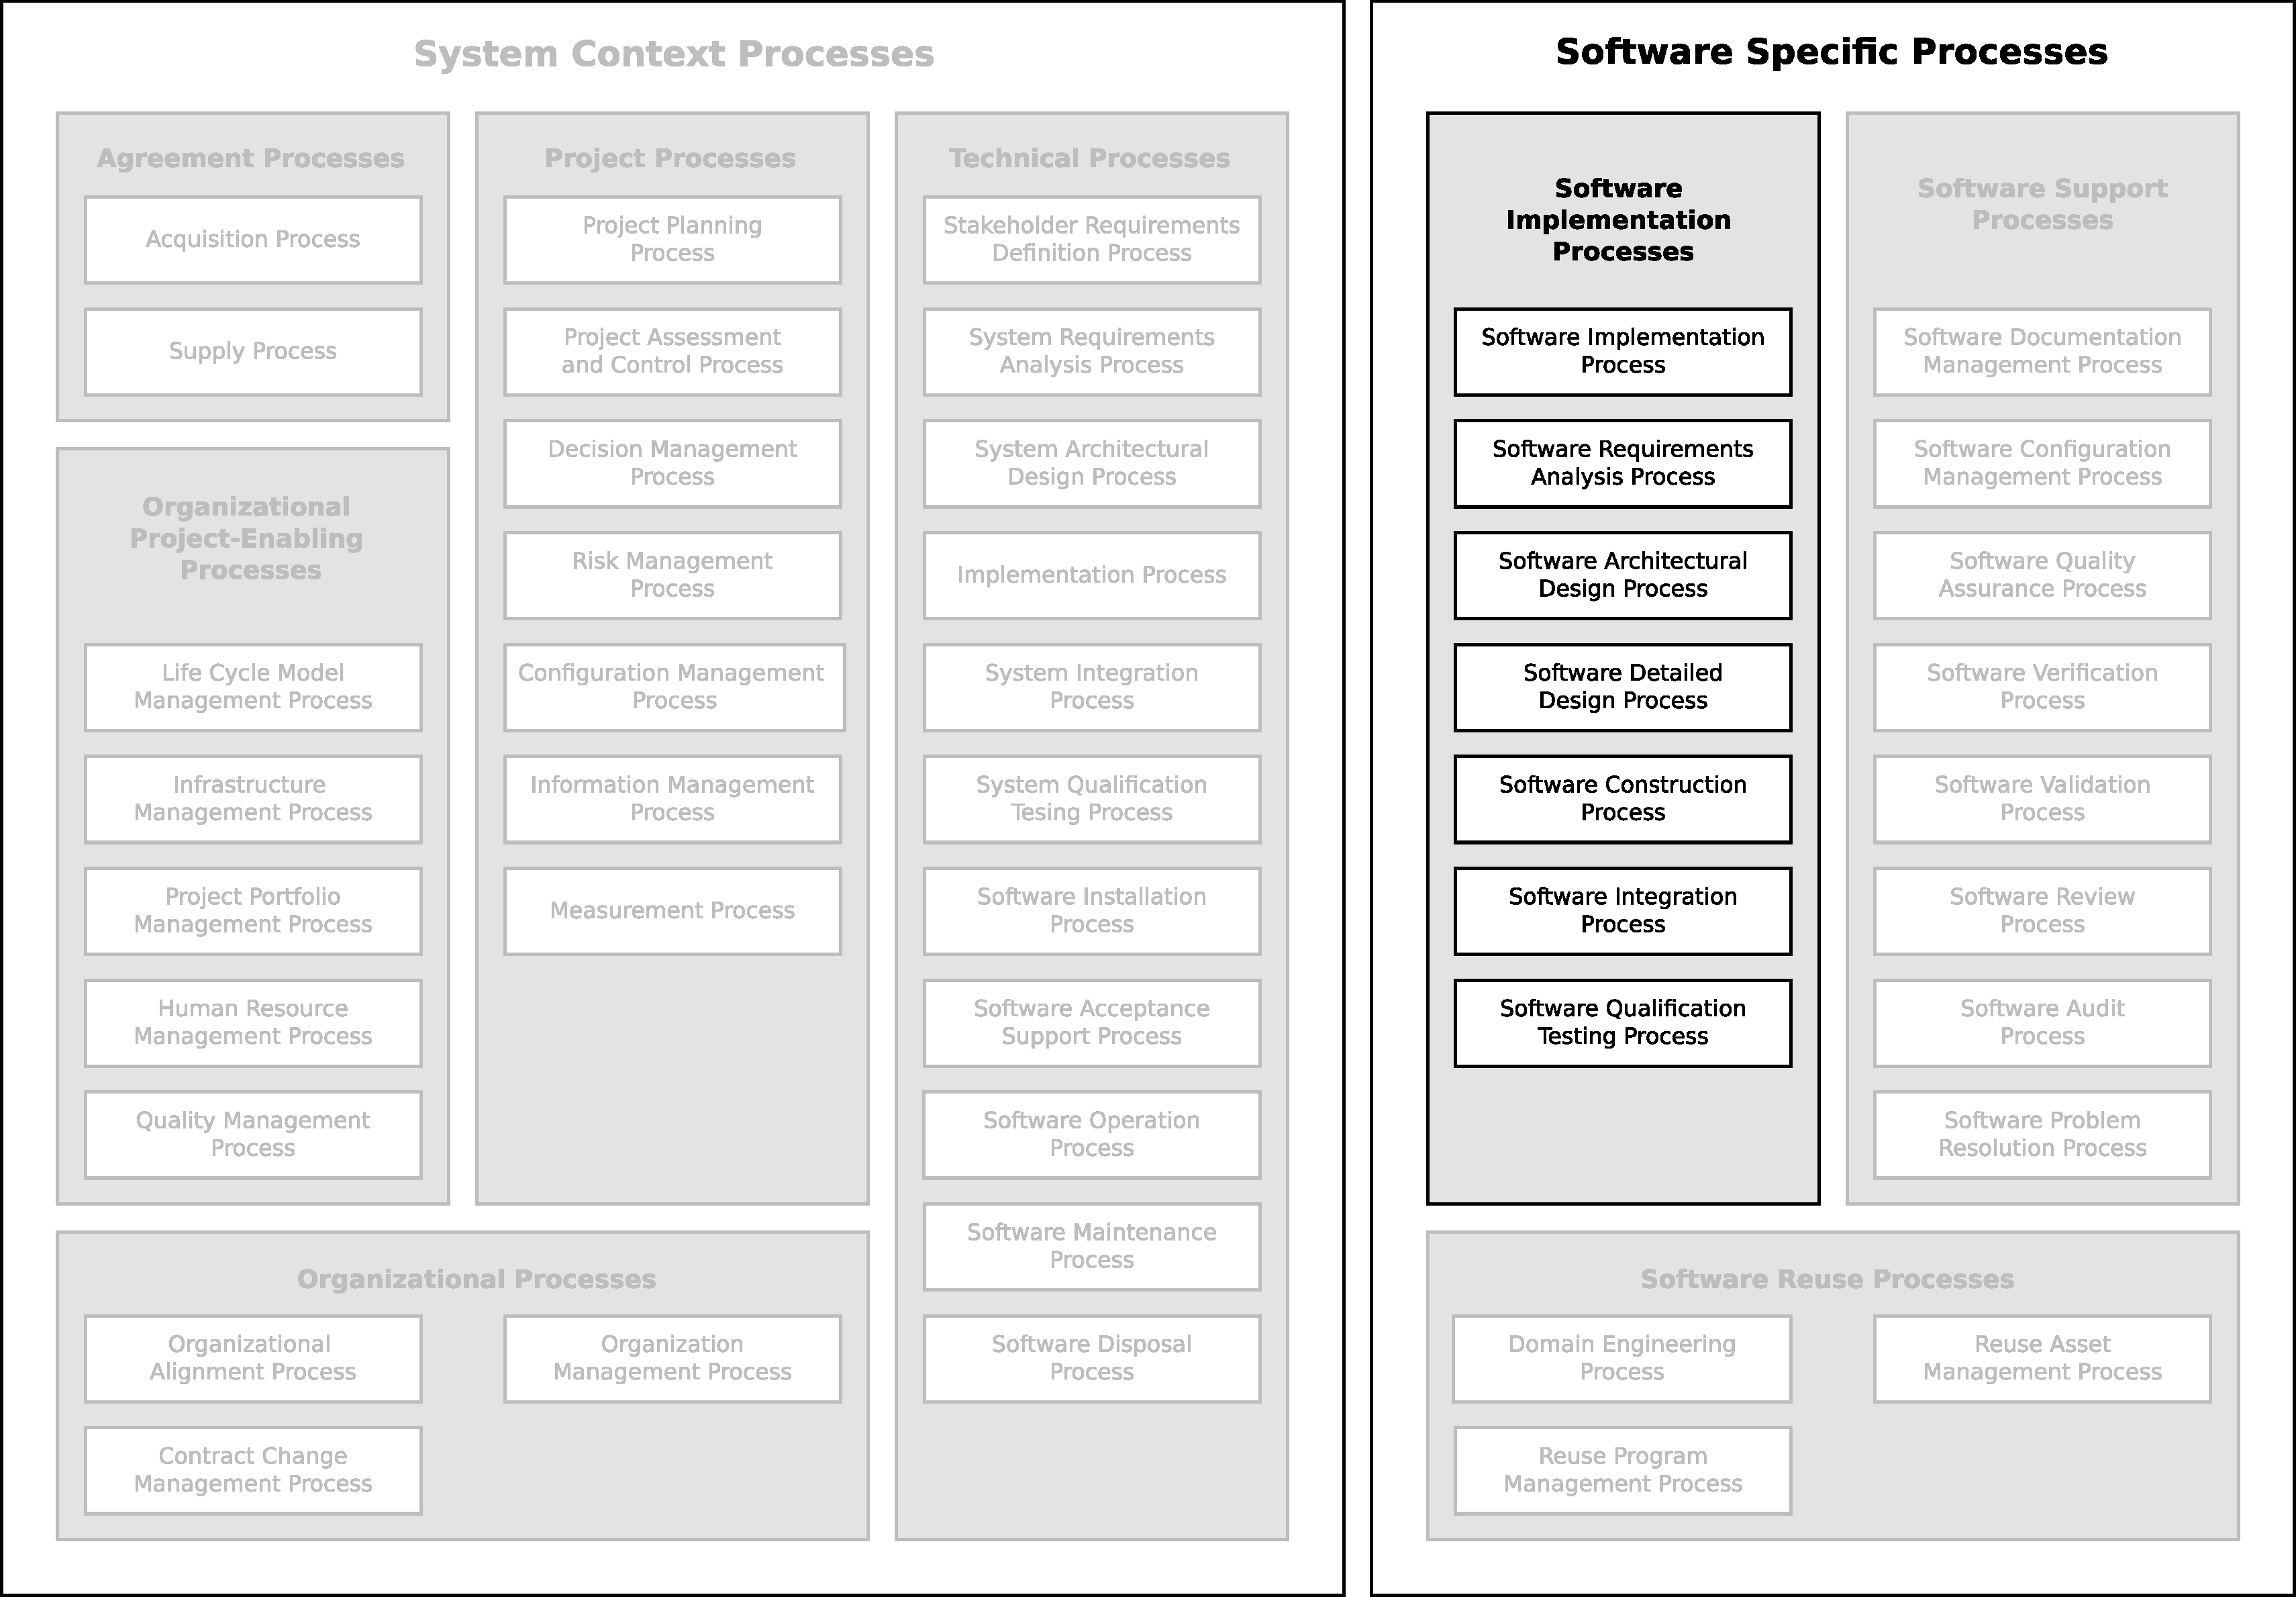
\includegraphics[width=15cm,keepaspectratio]{figures/life-cycle-process-groups-software-implementation-processes.pdf}
			\caption{Software Implementation Processes}
			\label{fig:software_implementation_processes}
		\end{figure}

		\begin{adjustwidth}{1em}{0pt}

			The \nameref{subsec:software_implementation_processes} are used to produce a specified system element (software item) implemented in software. Those processes transform specified behavior, interfaces and implementation constraints into implementation actions resulting in a system element that satisfies the requirements derived from the system requirements.

			\begin{compactitem}
				
				\item \ref{proc:software_implementation_process} - \nameref{proc:software_implementation_process}

				\item \ref{proc:software_requirements_analysis_process} - \nameref{proc:software_requirements_analysis_process}

				\item \ref{proc:software_architectural_design_process} - \nameref{proc:software_architectural_design_process}

				\item \ref{proc:software_detailed_design_process} - \nameref{proc:software_detailed_design_process}

				\item \ref{proc:software_construction_process} - \nameref{proc:software_detailed_design_process}

				\item \ref{proc:software_construction_process} - \nameref{proc:software_construction_process}

				\item \ref{proc:software_integration_process} - \nameref{proc:software_integration_process}

				\item \ref{proc:software_qualification_testing_process} - \nameref{proc:software_qualification_testing_process}

			\end{compactitem}

		\end{adjustwidth}

		\newpage
		\subsubsection{SOFTWARE IMPLEMENTATION PROCESS\label{proc:software_implementation_process}}

			\subsubsubsection{PURPOSE}
			\begin{adjustwidth}{2em}{0pt} 

				The purpose of the \nameref{proc:software_implementation_process} is to produce a specified system element implemented as a software product or service.

				This process transforms specified behavior, interfaces and implementation constraints into actions that create a system element implemented as a software product or service, otherwise known as a ``software item''. 

				This process results in a software item that satisfies architectural design requirements through verification and stakeholder requirements through validation.

			\end{adjustwidth}

			\subsubsubsection{OUTCOMES}
			\begin{adjustwidth}{2em}{0pt} 

				\begin{compactitem}

					\item an implementation strategy is defined;

					\item implementation technology constraints on the design are identified;

					\item a software item is realized; and

					\item a software item is packaged and stored in accordance with an agreement for its supply.

					\item In addition to its activities, this process has the following lower-level processes:

					\begin{compactenum}

						\item Software Architectural Design Process

						\item Software Detailed Design Process

						\item Software Construction Process

						\item Software Integration Process

						\item Software Qualification Testing Process

					\end{compactenum}

				\end{compactitem}

			\end{adjustwidth}

			\subsubsubsection{ACTIVITIES AND TASKS}
			\begin{adjustwidth}{2em}{0pt} 

				\begin{compactenum}

					\item {\bf Software Implementation Strategy}:

					\begin{compactenum}

						\item If not stipulated in the contract, the developer shall define or select a life cycle model appropriate to the scope, magnitude, and complexity of the project. The life cycle model shall be comprised of stages and the purpose and outcomes of each stage. The activities and tasks of the Software Implementation Process shall be selected and mapped onto the life cycle model.

						\item The implementer shall:

						\begin{compactenum}

							\item Document the outputs in accordance with the \nameref{proc:software_documentation_management_process}.

							\item Place the outputs under the \nameref{proc:software_configuration_management_process} and perform change control in accordance with it.

							\item Document and resolve problems and non-conformances found in the software products and tasks in accordance with the \nameref{proc:software_problem_resolution_process}.

							\item Perform supporting processes as specified in the contract.

							\item Establish baselines and incorporate configuration items at appropriate times, as determined by the acquirer and the supplier.

						\end{compactenum}

						\item The implementer shall select, tailor, and use those standards, methods, tools, and computer programming languages (if not stipulated in the contract) that are documented, appropriate, and established by the organization for performing the activities of the Software Implementation Process and supporting processes.

						\item The implementer shall develop plans for conducting the activities of the Software Implementation process. The plans should include specific standards, methods, tools, actions, and responsibility associated with the development and qualification of all requirements including safety and security. If necessary, separate plans may be developed. These plans shall be documented and executed.

						\item Non-deliverable items may be employed in the development or maintenance of the software product. However, it shall be ensured that the operation and maintenance of the deliverable software product after its delivery to the acquirer are independent of such items; otherwise, those items should be considered as deliverable.

					\end{compactenum}

				\end{compactenum}

			\end{adjustwidth}

		\newpage
		\subsubsection{SOFTWARE REQUIREMENTS ANALYSIS PROCESS\label{proc:software_requirements_analysis_process}}

			\subsubsubsection{PURPOSE}
			\begin{adjustwidth}{2em}{0pt} 

				The purpose of \nameref{proc:software_requirements_analysis_process} is to establish the requirements of the software elements of the system.

			\end{adjustwidth}

			\subsubsubsection{OUTCOMES}
			\begin{adjustwidth}{2em}{0pt} 

				\begin{compactitem}

					\item the requirements allocated to the software elements of the system and their interfaces are defined;

					\item software requirements are analyzed for correctness and testability;

					\item the impact of software requirements on the operating environment are understood;

					\item consistency and traceability are established between the software requirements and system requirements;

					\item prioritization for implementing the software requirements is defined;

					\item the software requirements are approved and updated as needed;

					\item changes to the software requirements are evaluated for cost, schedule and technical impact; and

					\item the software requirements are baselined and communicated to all affected parties.

				\end{compactitem}

			\end{adjustwidth}

			\subsubsubsection{ACTIVITIES AND TASKS}
			\begin{adjustwidth}{2em}{0pt} 

				\begin{compactenum}

					\item {\bf Software Requirements Analysis}:

					\begin{compactenum}

						\item The implementer shall establish and document software requirements (including the quality characteristics specifications) described below.

						\begin{compactenum}

							\item Functional and capability specifications, including performance, physical characteristics, environmental conditions under which the software item is to perform.

							\item Interfaces external to the software item.

							\item Qualification requirements.

							\item Safety specifications, including those related to methods of operation and maintenance, environmental influences, and personnel injury.

							\item Security specifications, including those related to compromise of sensitive information.

							\item Human-factors engineering (ergonomics) specifications, including those related to manual operations, human-equipment interactions, constraints on personnel, and areas needing concentrated human attention, that are sensitive to human errors and training.

							\item Data definition and database requirements.

							\item Installation and acceptance requirements of the delivered software product at the operation and maintenance site(s).

							\item User documentation requirements.

							\item User operation and execution requirements.

							\item User maintenance requirements.

						\end{compactenum}

						\item The implementer shall evaluate the software requirements considering the criteria listed below. The results of the evaluations shall be documented.

						\begin{compactenum}

							\item Traceability to system requirements and system design.

							\item External consistency with system requirements.

							\item Internal consistency.

							\item Testability.

							\item Feasibility of software design.

							\item Feasibility of operation and maintenance.

						\end{compactenum}

						\item The implementer shall conduct review(s) in accordance with \nameref{proc:software_review_process}.

					\end{compactenum}

				\end{compactenum}

			\end{adjustwidth}

		\newpage
		\subsubsection{SOFTWARE ARCHITECTURAL DESIGN PROCESS\label{proc:software_architectural_design_process}}

			\subsubsubsection{PURPOSE}
			\begin{adjustwidth}{2em}{0pt} 
				
				The purpose of the \nameref{proc:software_architectural_design_process} is to provide a design for the software that implements and can be verified against the requirements.

			\end{adjustwidth}

			\subsubsubsection{OUTCOMES}
			\begin{adjustwidth}{2em}{0pt} 

				\begin{compactitem}

					\item a software architectural design is developed and baselined that describes the software items that will implement the software requirements;

					\item internal and external interfaces of each software item are defined; and

					\item consistency and traceability are established between software requirements and software design.

				\end{compactitem}

			\end{adjustwidth}

			\subsubsubsection{ACTIVITIES AND TASKS}
			\begin{adjustwidth}{2em}{0pt} 

				\begin{compactenum}

					\item {\bf Software Architectural Design}:

					\begin{compactenum}

						\item The implementer shall transform the requirements for the software item into an architecture that describes its top-level structure and identifies the software components. It shall be ensured that all the requirements for the software item are allocated to its software components and further refined to facilitate detailed design. The architecture of the software item shall be documented.

						\item The implementer shall develop and document a top-level design for the interfaces external to the software item and between the software components of the software item.

						\item The implementer shall develop and document a top-level design for the database.

						\item The implementer should develop and document preliminary versions of user documentation.

						\item The implementer shall define and document preliminary test requirements and the schedule for Software Integration.

						\item The implementer shall evaluate the architecture of the software item and the interface and database designs considering the criteria listed below. The results of the evaluations shall be documented.

						\begin{compactenum}

							\item Traceability to the requirements of the software item.

							\item External consistency with the requirements of the software item.

							\item Internal consistency between the software components.

							\item Appropriateness of design methods and standards used.

							\item Feasibility of detailed design.

							\item Feasibility of operation and maintenance.

						\end{compactenum}

						\item The implementer shall conduct review(s) in accordance with \nameref{proc:software_review_process}

					\end{compactenum}

				\end{compactenum}

			\end{adjustwidth}

		\newpage
		\subsubsection{SOFTWARE DETAILED DESIGN PROCESS\label{proc:software_detailed_design_process}}

			\subsubsubsection{PURPOSE}
			\begin{adjustwidth}{2em}{0pt} 

				The purpose of the \nameref{proc:software_detailed_design_process} is to provide a design for the software that implements and can be verified against the requirements and the software architecture and is sufficiently detailed to permit coding and testing.

			\end{adjustwidth}

			\subsubsubsection{OUTCOMES}
			\begin{adjustwidth}{2em}{0pt} 

				\begin{compactitem}

					\item a detailed design of each software component, describing the software units to be built, is developed;

					\item external interfaces of each software unit are defined; and

					\item consistency and traceability are established between the detailed design and the requirements and architectural design.

				\end{compactitem}

			\end{adjustwidth}

			\subsubsubsection{ACTIVITIES AND TASKS}
			\begin{adjustwidth}{2em}{0pt} 

				\begin{compactenum}

					\item {\bf Software Detailed Design}:

					\begin{compactenum}

						\item The implementer shall develop a detailed design for each software component of the software item. The software components shall be refined into lower levels containing software units that can be coded, compiled, and tested. It shall be ensured that all the software requirements are allocated from the software components to software units. The detailed design shall be documented.

						\item The implementer shall develop and document a detailed design for the interfaces external to the software item, between the software components, and between the software units. The detailed design of the interfaces shall permit coding without the need for further information.

						\item The implementer shall develop and document a detailed design for the database.

						\item The implementer shall update user documentation as necessary.

						\item The implementer shall define and document test requirements and the schedule for testing software units. The test requirements should include stressing the software unit at the limits of its requirements.

						\item The implementer shall update the test requirements and the schedule for Software Integration.

						\item The implementer shall evaluate the software detailed design and test requirements considering the criteria listed below. The results of the evaluations shall be documented.

						\begin{compactenum}

							\item Traceability to the requirements of the software item;

							\item External consistency with architectural design;

							\item Internal consistency between software components and software units;

							\item Appropriateness of design methods and standards used;

							\item Feasibility of testing;

							\item Feasibility of operation and maintenance.

						\end{compactenum}

						\item The implementer shall conduct review(s) in accordance with the \nameref{proc:software_review_process}.

					\end{compactenum}

				\end{compactenum}

			\end{adjustwidth}

		\newpage
		\subsubsection{SOFTWARE CONSTRUCTION PROCESS\label{proc:software_construction_process}}

			\subsubsubsection{PURPOSE}
			\begin{adjustwidth}{2em}{0pt} 
				
				The purpose of the \nameref{proc:software_construction_process} is to produce executable software units that properly reflect the software design.

			\end{adjustwidth}

			\subsubsubsection{OUTCOMES}
			\begin{adjustwidth}{2em}{0pt} 

				\begin{compactitem}

					\item verification criteria are defined for all software units against their requirements;

					\item software units defined by the design are produced;

					\item consistency and traceability are established between software units and requirements and design; and

					\item verification of the software units against the requirements and the design is accomplished.

				\end{compactitem}

			\end{adjustwidth}

			\subsubsubsection{ACTIVITIES AND TASKS}
			\begin{adjustwidth}{2em}{0pt} 

				\begin{compactenum}

					\item {\bf Software Construction}:

					\begin{compactenum}

						\item The implementer shall develop and document the following:

						\item Each software unit and database.

						\item Test procedures and data for testing each software unit and database.

						\item The implementer shall test each software unit and database ensuring that it satisfies its requirements. The test results shall be documented.

						\item The implementer shall update the user documentation as necessary.

						\item The implementer shall update the test requirements and the schedule for Software Integration.

						\item The implementer shall evaluate software code and test results considering the criteria listed below. The results of the evaluations shall be documented.

						\begin{compactenum}

							\item Traceability to the requirements and design of the software item.

							\item External consistency with the requirements and design of the software item.

							\item Internal consistency between unit requirements.

							\item Test coverage of units.

							\item Appropriateness of coding methods and standards used.

							\item Feasibility of software integration and testing.

							\item Feasibility of operation and maintenance.

						\end{compactenum}

					\end{compactenum}

				\end{compactenum}

			\end{adjustwidth}

		\newpage
		\subsubsection{SOFTWARE INTEGRATION PROCESS\label{proc:software_integration_process}}

			\subsubsubsection{PURPOSE}
			\begin{adjustwidth}{2em}{0pt} 

				The purpose of the \nameref{proc:software_integration_process} is to combine the software units and software components, producing integrated software items, consistent with the software design, that demonstrate that the functional and non-functional software requirements are satisfied on an equivalent or complete operational platform.

			\end{adjustwidth}

			\subsubsubsection{OUTCOMES}
			\begin{adjustwidth}{2em}{0pt} 

				\begin{compactitem}

					\item an integration strategy is developed for software units consistent with the software design and the prioritized software requirements;

					\item verification criteria for software items are developed that ensure compliance with the software requirements allocated to the items;

					\item software items are verified using the defined criteria;

					\item software items defined by the integration strategy are produced;

					\item results of integration testing are recorded;

					\item consistency and traceability are established between software design and software items; and

					\item a regression strategy is developed and applied for re-verifying software items when a change in software units (including associated requirements, design and code) occur.

				\end{compactitem}

			\end{adjustwidth}

			\subsubsubsection{ACTIVITIES AND TASKS}
			\begin{adjustwidth}{2em}{0pt} 

				\begin{compactenum}

					\item {\bf Software Integration}:

					\begin{compactenum}

						\item The implementer shall develop an integration plan to integrate the software units and software components into the software item. The plan shall include test requirements, procedures, data, responsibilities, and schedule. The plan shall be documented.

						\item The implementer shall integrate the software units and software components and test as the aggregates are developed in accordance with the integration plan. It shall be ensured that each aggregate satisfies the requirements of the software item and that the software item is integrated at the conclusion of the integration activity. The integration and test results shall be documented.


						\item The implementer shall update the user documentation as necessary.

						\item The implementer shall develop and document for each qualification requirement of the software item a set of tests, test cases (inputs, outputs, test criteria), and test procedures for conducting Software Qualification Testing. The developer shall ensure that the integrated software item is ready for Software Qualification Testing.

						\item The implementer shall evaluate the integration plan, design, code, tests, test results, and user documentation considering the criteria listed below. The results of the evaluations shall be documented.

						\begin{compactenum}

							\item Traceability to the system requirements.

							\item External consistency with the system requirements.

							\item Internal consistency.

							\item Test coverage of the requirements of the software item.

							\item Appropriateness of test standards and methods used.

							\item Conformance to expected results.

							\item Feasibility of software qualification testing.

							\item Feasibility of operation and maintenance.

						\end{compactenum}

					\end{compactenum}

				\end{compactenum}

			\end{adjustwidth}

		\newpage
		\subsubsection{SOFTWARE QUALIFICATION TESTING PROCESS\label{proc:software_qualification_testing_process}}

			\subsubsubsection{PURPOSE}
			\begin{adjustwidth}{2em}{0pt} 

				The purpose of the \nameref{proc:software_qualification_testing_process} is to confirm that the integrated software product meets its defined requirements.

			\end{adjustwidth}

			\subsubsubsection{OUTCOMES}
			\begin{adjustwidth}{2em}{0pt} 

				\begin{compactitem}

					\item criteria for the integrated software is developed that demonstrates compliance with the software requirements;

					\item integrated software is verified using the defined criteria;

					\item test results are recorded; and

					\item a regression strategy is developed and applied for re-testing the integrated software when a change in software items is made.

				\end{compactitem}

			\end{adjustwidth}

			\subsubsubsection{ACTIVITIES AND TASKS}
			\begin{adjustwidth}{2em}{0pt} 

				\begin{compactenum}

					\item {\bf Software Qualification Testing}:

					\begin{compactenum}

						\item The implementer shall conduct qualification testing in accordance with the qualification requirements for the software item. It shall be ensured that the implementation of each software requirement is tested for compliance. The qualification testing results shall be documented.

						\item The implementer shall update the user documentation as necessary.

						\item The implementer shall evaluate the design, code, tests, test results, and user documentation considering the criteria listed below. The results of the evaluations shall be documented.

						\begin{compactenum}

							\item Test coverage of the requirements of the software item.

							\item Conformance to expected results.

							\item Feasibility of system integration and testing, if conducted.

							\item Feasibility of operation and maintenance.

						\end{compactenum}

						\item The implementer shall support audit(s) in accordance with the \nameref{proc:software_audit_process}. The results of the audits shall be documented. If both hardware and software are under development or integration, the audits may be postponed until the System Qualification Testing.

						\item Upon successful completion of the audits, if conducted, the implementer shall update and prepare the deliverable software product for the \nameref{proc:system_integration_process}, \nameref{proc:system_qualification_testing_process}, \nameref{proc:software_installation_process}, or \nameref{proc:software_acceptance_support_process} accordingly.

					\end{compactenum}

				\end{compactenum}

			\end{adjustwidth}

	\newpage 
	\subsection{SOFTWARE SUPPORT PROCESSES\label{subsec:software_support_processes}}

		\begin{figure}[h]
			\centering
			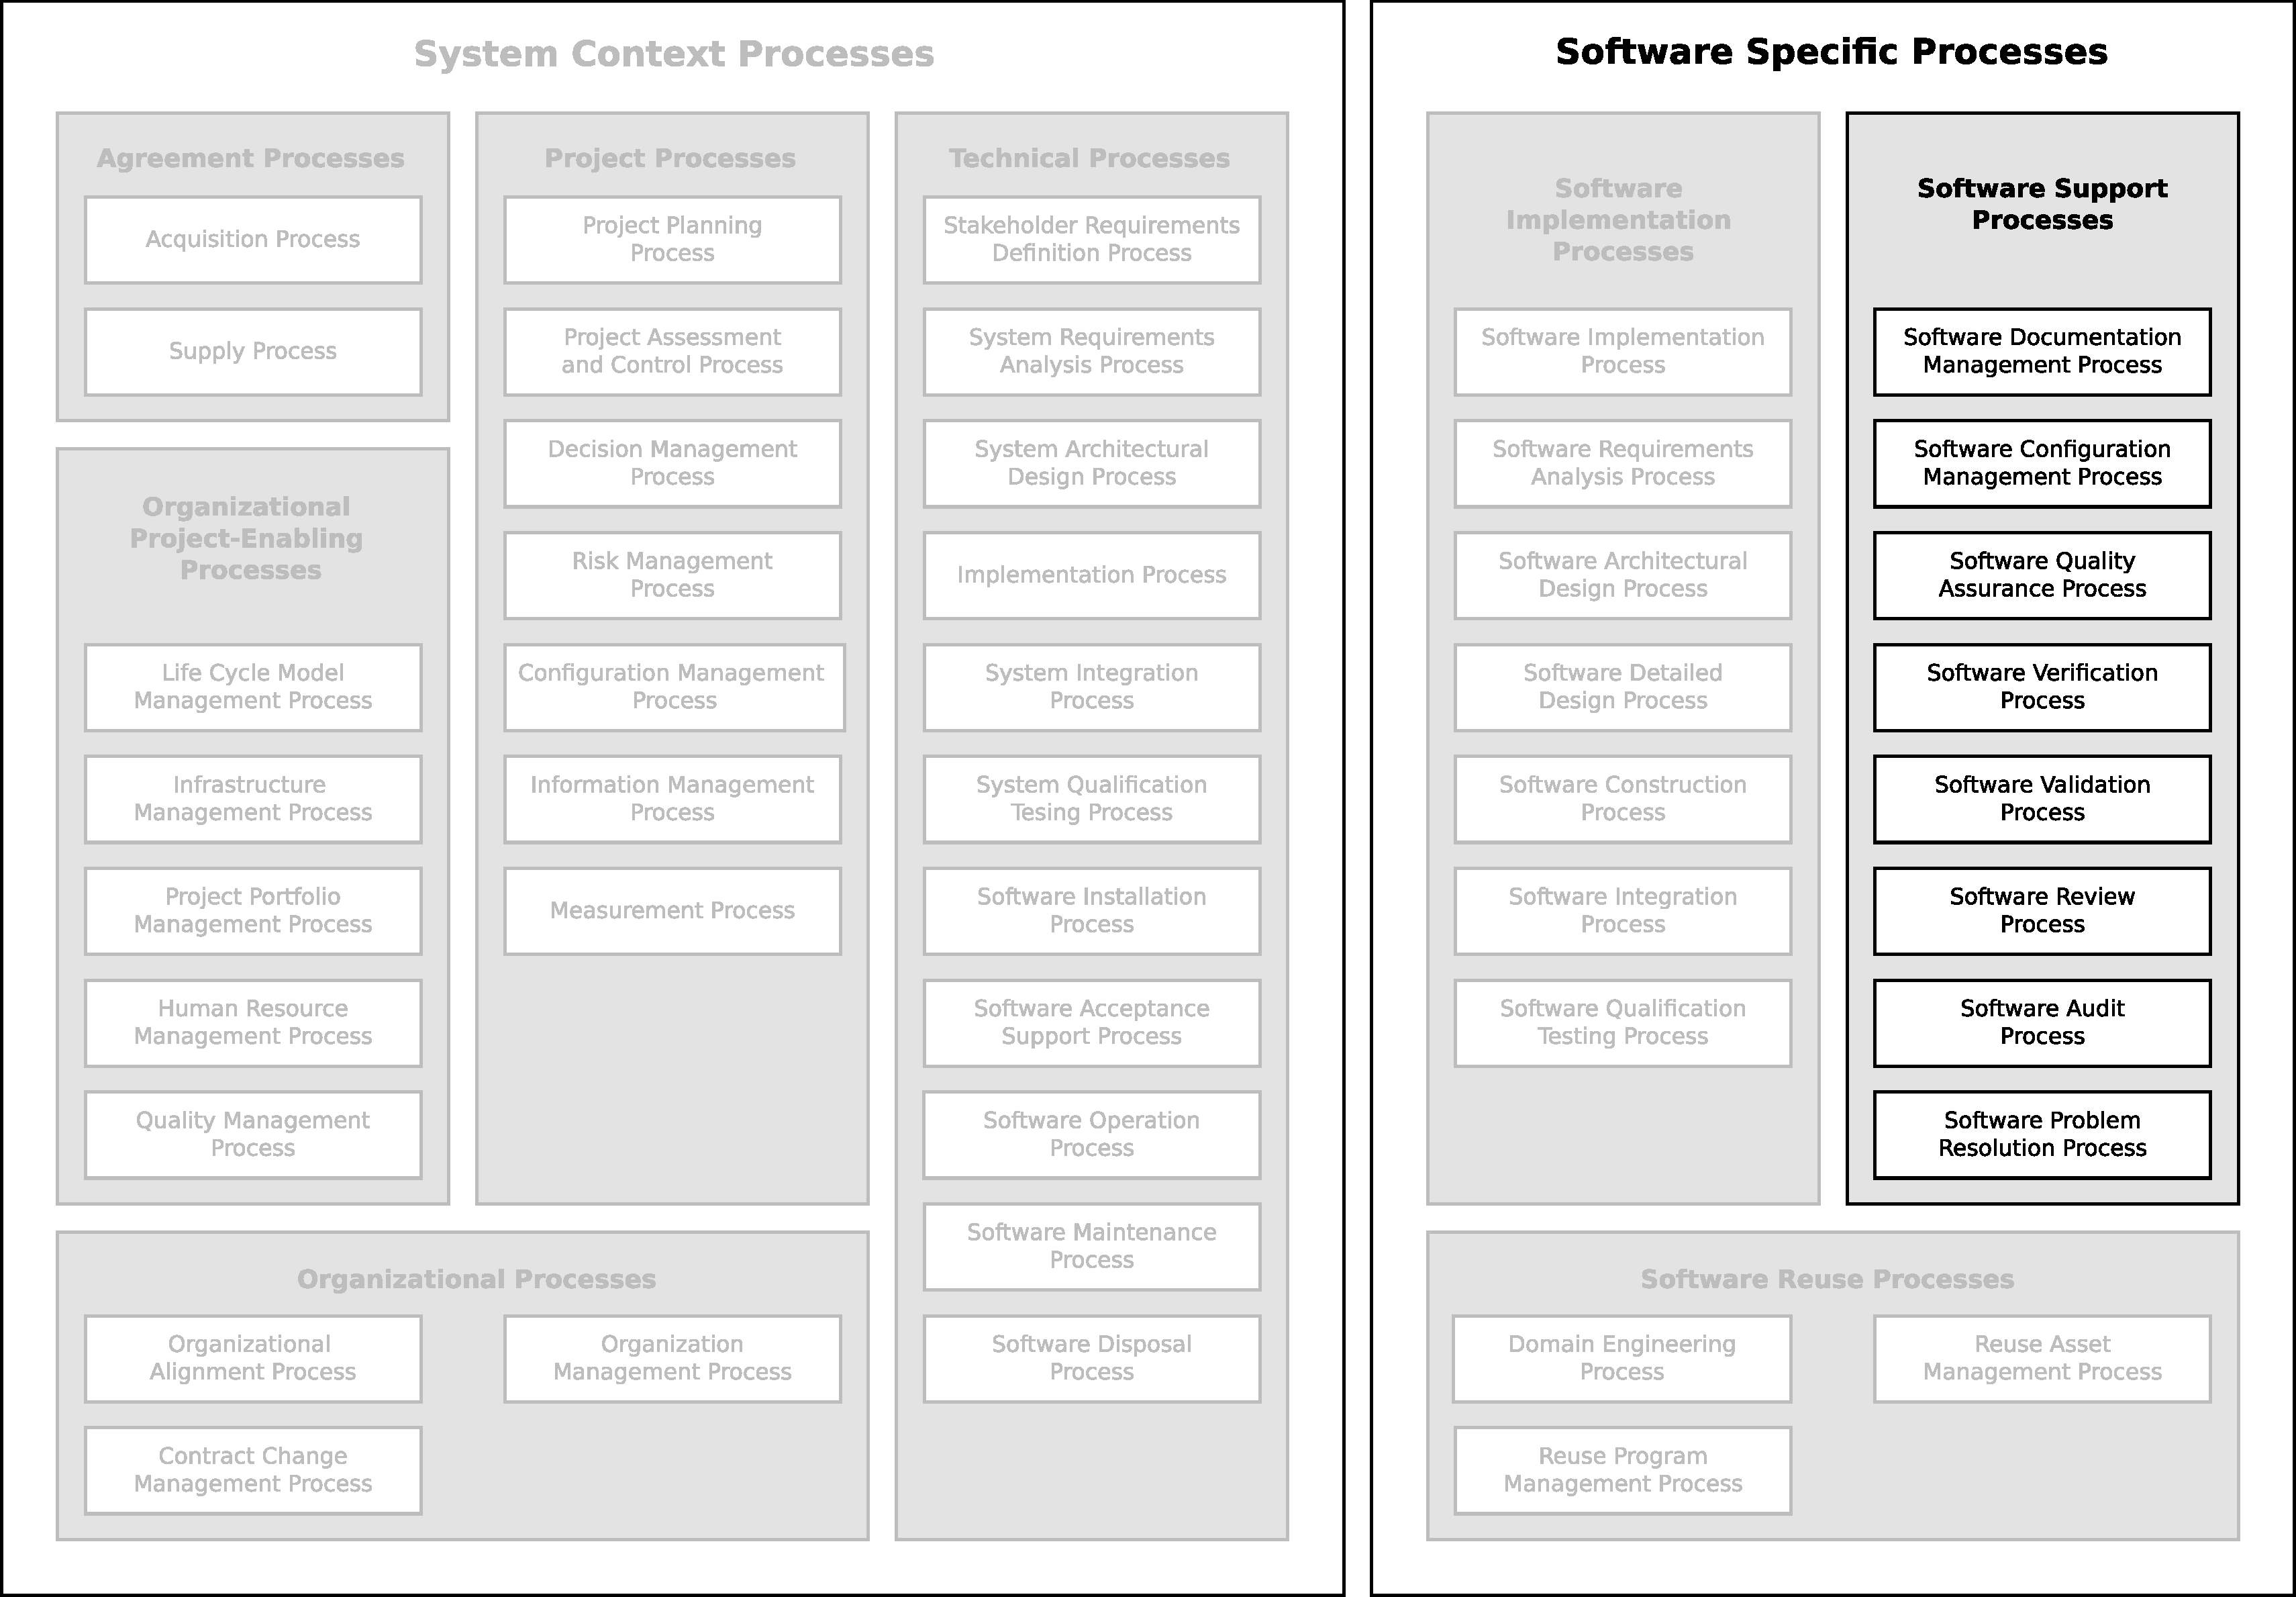
\includegraphics[width=15cm,keepaspectratio]{figures/life-cycle-process-groups-software-support-processes.pdf}
			\caption{Software Support Processes}
			\label{fig:software_support_processes}
		\end{figure}

		\begin{adjustwidth}{1em}{0pt}
			
			{\bf Note}: The support processes listed in this section are specific to software and are labeled \nameref{subsec:software_support_processes}. Although they play an integral role in assisting the \nameref{proc:software_implementation_process}, the Software Support Processes may also provide services to other processes, e.g., the \nameref{subsec:agreement_processes}, \nameref{proc:system_qualification_testing_process}, \nameref{proc:software_acceptance_support_process}, \nameref{proc:software_operation_process}, and \nameref{proc:software_maintenance_process}.

			\begin{compactitem}

				\item \ref{proc:software_documentation_management_process} - \nameref{proc:software_documentation_management_process}

				\item \ref{proc:software_configuration_management_process} - \nameref{proc:software_configuration_management_process}

				\item \ref{proc:software_quality_assurance_process} - \nameref{proc:software_quality_assurance_process}

				\item \ref{proc:software_verification_process} - \nameref{proc:software_verification_process}

				\item \ref{proc:software_validation_process} - \nameref{proc:software_validation_process}

				\item \ref{proc:software_review_process} - \nameref{proc:software_review_process}

				\item \ref{proc:software_audit_process} - \nameref{proc:software_audit_process}

				\item \ref{proc:software_problem_resolution_process} - \nameref{proc:software_problem_resolution_process}

			\end{compactitem}

		\end{adjustwidth}

		\newpage
		\subsubsection{SOFTWARE DOCUMENTATION MANAGEMENT PROCESS\label{proc:software_documentation_management_process}}

			\subsubsubsection{PURPOSE}
			\begin{adjustwidth}{2em}{0pt} 

				The purpose of the \nameref{proc:software_documentation_management_process} is to develop and maintain the recorded software information produced by a process.

			\end{adjustwidth}

			\subsubsubsection{OUTCOMES}
			\begin{adjustwidth}{2em}{0pt} 

				\begin{compactitem}

					\item a strategy identifying the documentation to be produced during the life cycle of the software product or service is developed;

					\item the standards to be applied for the development of the software documentation are identified;

					\item documentation to be produced by the process or project is identified;

					\item the content and purpose of all documentation is specified, reviewed and approved;

					\item documentation is developed and made available in accordance with identified standards; and

					\item documentation is maintained in accordance with defined criteria.

				\end{compactitem}

			\end{adjustwidth}

			\subsubsubsection{ACTIVITIES AND TASKS}
			\begin{adjustwidth}{2em}{0pt} 

				\begin{compactenum}

					\item {\bf Process Implementation}:
					\begin{compactenum}

						\item A plan, identifying the documents to be produced during the life cycle of the software product shall be developed, documented, and implemented. For identified documentation, the following shall be addressed:

						\begin{compactenum}

							\item Title or name.

							\item Purpose and content.

							\item Intended audience.

							\item Procedures and responsibilities for inputs, development, review, modification, approval, production,
							storage, distribution, maintenance, and configuration management.

							\item Schedule for intermediate and final versions.

						\end{compactenum}

					\end{compactenum}

					\item {\bf Design and Development}:
					\begin{compactenum}

						\item Each identified document shall be designed in accordance with applicable documentation standards for medium, format, content description, page numbering, figure/table placement, proprietary/security marking, packaging, and other presentation items.

						\item The source and appropriateness of input data for the documents shall be confirmed. Automated documentation support tools may be used.

						\item The prepared documents shall be reviewed and edited for format, technical content, and presentation style against their documentation standards. They shall be approved for adequacy by authorized personnel prior to issue.

					\end{compactenum}

					\item {\bf Production}:
					\begin{compactenum}

						\item The documents shall be produced and provided in accordance with the plan. Production and distribution of documents may use paper, electronic, or other media. Master materials shall be stored in accordance with requirements for record retention, security, maintenance, and backup.

						\item Controls shall be established in accordance with the \nameref{proc:software_configuration_management_process}.

					\end{compactenum}

					\item {\bf Maintenance}:
					\begin{compactenum}

						\item The tasks of the \nameref{proc:software_maintenance_process}, that are required when documentation is to be modified, shall be performed. For those documents that are under configuration management, modifications shall be managed in accordance with the \nameref{proc:software_configuration_management_process}.

					\end{compactenum}

				\end{compactenum}

			\end{adjustwidth}

		\newpage
		\subsubsection{SOFTWARE CONFIGURATION MANAGEMENT PROCESS\label{proc:software_configuration_management_process}}

			\subsubsubsection{PURPOSE}
			\begin{adjustwidth}{2em}{0pt} 

				The purpose of the \nameref{proc:software_configuration_management_process} is to establish and maintain the integrity of the software items of a process or project and make them available to concerned parties.

			\end{adjustwidth}

			\subsubsubsection{OUTCOMES}
			\begin{adjustwidth}{2em}{0pt} 

				\begin{compactitem}

					\item a software configuration management strategy is developed;

					\item items generated by the process or project are identified, defined and baselined;

					\item modifications and releases of the items are controlled;

					\item modifications and releases are made available to affected parties;

					\item the status of the items and modifications are recorded and reported;

					\item the completeness and consistency of the items is ensured; and

					\item the storage, handling and delivery of the items are controlled.

				\end{compactitem}

			\end{adjustwidth}

			\subsubsubsection{ACTIVITIES AND TASKS}
			\begin{adjustwidth}{2em}{0pt} 

				\begin{compactenum}

					\item {\bf Process Implementation}:

					\begin{compactenum}

						\item A software configuration management plan shall be developed. The plan shall describe: the configuration management activities; procedures and schedule for performing these activities; the organization(s) responsible for performing these activities; and their relationship with other organizations, such as software development or maintenance. The plan shall be documented and implemented.

					\end{compactenum}

					\item {\bf Configuration Identification}:

					\begin{compactenum}

						\item A scheme shall be established for identification of software items and their versions to be controlled for the project. For each software item and its versions, the following shall be identified: the documentation that establishes the baseline; the version references; and other identification details.

					\end{compactenum}

					\item {\bf Configuration Control}:

					\begin{compactenum}

						\item The following shall be performed: identification and recording of change requests; analysis and evaluation of the changes; approval or disapproval of the request; and implementation, verification, and release of the modified software item. An audit trail shall exist, whereby each modification, the reason for the modification, and authorization of the modification can be traced. Control and audit of all accesses to the controlled software items that handle safety or security critical functions shall be performed.

					\end{compactenum}

					\item {\bf Configuration Status Accounting}:

					\begin{compactenum}

						\item Management records and status reports that show the status and history of controlled software items, including baselines shall be prepared. Status reports should include the number of changes for a project, latest software item versions, release identifiers, the number of releases, and comparisons of releases.

					\end{compactenum}

					\item {\bf Configuration Evaluation}:

					\begin{compactenum}

						\item The following shall be determined and ensured: the functional completeness of the software items against their requirements and the physical completeness of the software items (whether their design and code reflect an up-to-date technical description).

					\end{compactenum}

					\item {\bf Release Management and Delivery}:

					\begin{compactenum}

						\item The release and delivery of software products and documentation shall be formally controlled. Master copies of code and documentation shall be maintained for the life of the software product. The code and documentation that contain safety or security critical functions shall be handled, stored, packaged, and delivered in accordance with the policies of the organizations involved.

					\end{compactenum}

				\end{compactenum}

			\end{adjustwidth}

		\newpage
		\subsubsection{SOFTWARE QUALITY ASSURANCE PROCESS\label{proc:software_quality_assurance_process}}

			\subsubsubsection{PURPOSE}
			\begin{adjustwidth}{2em}{0pt} 

				The purpose of the \nameref{proc:software_quality_assurance_process} is to provide assurance that work products and processes comply with predefined provisions and plans.

			\end{adjustwidth}

			\subsubsubsection{OUTCOMES}
			\begin{adjustwidth}{2em}{0pt} 

				\begin{compactitem}

					\item a strategy for conducting quality assurance is developed;

					\item evidence of software quality assurance is produced and maintained;

					\item problems and/or non-conformance with requirements are identified and recorded; and

					\item adherence of products, processes and activities to the applicable standards, procedures and requirements are verified.

				\end{compactitem}

			\end{adjustwidth}

			\subsubsubsection{ACTIVITIES AND TASKS}
			\begin{adjustwidth}{2em}{0pt} 

				\begin{compactenum}

					\item {\bf Process Implementation}:

					\begin{compactenum}

						\item A quality assurance process suited to the project shall be established. The objectives of the quality assurance process shall be to assure that the software products and the processes employed for providing those software products comply with their established requirements and adhere to their established plans.

						\item The quality assurance process should be coordinated with the related \nameref{proc:software_verification_process}, \nameref{proc:software_validation_process}, \nameref{proc:software_review_process}, and \nameref{proc:software_audit_process}.

						\item A plan for conducting the quality assurance process activities and tasks shall be developed, documented, implemented, and maintained for the life of the contract. The plan shall include the following:

						\begin{compactenum}

							\item Quality standards, methodologies, procedures, and tools for performing the quality assurance activities (or their references in organization's official documentation).

							\item Procedures for contract review and coordination thereof.

							\item Procedures for identification, collection, filing, maintenance, and disposition of quality records.

							\item Resources, schedule, and responsibilities for conducting the quality assurance activities.

							\item Selected activities and tasks from supporting processes, such as the \nameref{proc:software_verification_process}, \nameref{proc:software_validation_process}, \nameref{proc:software_review_process}, \nameref{proc:software_audit_process}, and \nameref{proc:software_problem_resolution_process}.

						\end{compactenum}

							\item Scheduled and on-going quality assurance activities and tasks shall be executed. When problems or non-conformances with contract requirements are detected, they shall be documented and serve as input to the \nameref{proc:software_problem_resolution_process}. Records of these activities and tasks, their execution, problems, and problem resolutions shall be prepared and maintained.

							\item Records of quality assurance activities and tasks shall be made available to the acquirer as specified in the contract.

							\item It shall be assured that persons responsible for assuring compliance with the contract requirements have the organizational freedom, resources, and authority to permit objective evaluations and to initiate, effect, resolve, and verify problem resolutions.

					\end{compactenum}

					\item {\bf Product Assurance}:

					\begin{compactenum}

						\item It shall be assured that all the plans required by the contract are documented, comply with the contract, are mutually consistent, and are being executed as required.

						\item It shall be assured that software products and related documentation comply with the contract and adhere to the plans.

						\item In preparation for the delivery of the software products, it shall be assured that they have fully satisfied their contractual requirements and are acceptable to the acquirer.

					\end{compactenum}

					\item {\bf Process Assurance}:

					\begin{compactenum}

						\item It shall be assured that those software life cycle processes (supply, development, operation, maintenance, and support processes including quality assurance) employed for the project comply with the contract and adhere to the plans.

						\item It shall be assured that the internal software engineering practices, development environment, test environment, and libraries comply with the contract.

						\item It shall be assured that applicable prime-contract requirements are passed down to the subcontractor, and that the subcontractor's software products satisfy prime-contract requirements.

						\item It shall be assured that the acquirer and other parties are provided the required support and cooperation in accordance with the contract, negotiations, and plans.

						\item It should be assured that software product and process measurements are in accordance with established standards and procedures.

						\item It shall be assured that the staff assigned have the skill and knowledge needed to meet the requirements of the project and receive any necessary training.

					\end{compactenum}

				\end{compactenum}

			\end{adjustwidth}

		\newpage
		\subsubsection{SOFTWARE VERIFICATION PROCESS\label{proc:software_verification_process}}

			\subsubsubsection{PURPOSE}
			\begin{adjustwidth}{2em}{0pt} 

				The purpose of the \nameref{proc:software_verification_process} is to confirm that each software work product and/or service of a process or project properly reflects the specified requirements.

			\end{adjustwidth}

			\subsubsubsection{OUTCOMES}
			\begin{adjustwidth}{2em}{0pt} 

				\begin{compactitem}

					\item a verification strategy is developed and implemented;

					\item criteria for verification of all required software work products is identified;

					\item required verification activities are performed;

					\item defects are identified and recorded; and

					\item results of the verification activities are made available to the customer and other involved parties.

				\end{compactitem}

			\end{adjustwidth}

			\subsubsubsection{ACTIVITIES AND TASKS}
			\begin{adjustwidth}{2em}{0pt} 

				\begin{compactenum}

					\item {\bf Process Implementation}:

					\begin{compactenum}

						\item A determination shall be made if the project warrants a verification effort and the degree of organizational independence of that effort needed. The project requirements shall be analyzed for criticality. Criticality may be gauged in terms of:

						\begin{compactenum}

							\item The potential of an undetected error in a system or software requirement for causing death or personal injury, mission failure, or financial or catastrophic equipment loss or damage.

							\item The maturity of and risks associated with the software technology to be used.

							\item Availability of funds and resources.

						\end{compactenum}

						\item If the project warrants a verification effort, a verification process shall be established to verify the software product.

						\item If the project warrants an independent verification effort, a qualified organization responsible for conducting the verification shall be selected. This organization shall be assured of the independence and authority to perform the verification activities.

						\item Based upon the scope, magnitude, complexity, and criticality analysis above, target life cycle activities and software products requiring verification shall be determined. Verification activities and tasks defined in the \nameref{proc:software_verification_process}, including associated methods, techniques, and tools for performing the tasks, shall be selected for the target life cycle activities and software products.

						\item Based upon the verification tasks as determined, a verification plan shall be developed and documented. The plan shall address the life cycle activities and software products subject to verification, the required verification tasks for each life cycle activity and software product, and related resources, responsibilities, and schedule. The plan shall address procedures for forwarding verification reports to the acquirer and other involved organizations.

						\item The verification plan shall be implemented. Problems and non-conformances detected by the verification effort shall be entered into the \nameref{proc:software_problem_resolution_process}. All problems and non-conformances shall be resolved. Results of the verification activities shall be made available to the acquirer and other involved organizations.

					\end{compactenum}

					\item {\bf Requirements Verification}:

					\begin{compactenum}

						\item The system requirements are consistent, feasible, and testable.

						\item The system requirements have been appropriately allocated to hardware items, software items, and manual operations according to design criteria.

						\item The software requirements are consistent, feasible, testable, and accurately reflect system requirements.

						\item The software requirements related to safety, security, and criticality are correct as shown by suitably rigorous methods.

					\end{compactenum}

					\item {\bf Design Verification}:

					\begin{compactenum}

						\item The design is correct and consistent with and traceable to requirements.

						\item The design implements proper sequence of events, inputs, outputs, interfaces, logic flow, allocation of timing and sizing budgets, and error definition, isolation, and recovery.

						\item Selected design can be derived from requirements.

						\item The design implements safety, security, and other critical requirements correctly as shown by suitably rigorous methods.

					\end{compactenum}

					\item {\bf Code Verification}:

					\begin{compactenum}

						\item The code is traceable to design and requirements, testable, correct, and compliant with requirements and coding standards.

						\item The code implements proper event sequence, consistent interfaces, correct data and control flow, completeness, appropriate allocation timing and sizing budgets, and error definition, isolation, and recovery.

						\item Selected code can be derived from design or requirements.

						\item The code implements safety, security, and other critical requirements correctly as shown by suitably rigorous methods.

					\end{compactenum}

					\item {\bf Integration Verification}:

					\begin{compactenum}

						\item The software components and units of each software item have been completely and correctly integrated into the software item.

						\item The hardware items, software items, and manual operations of the system have been completely and correctly integrated into the system.

						\item The integration tasks have been performed in accordance with an integration plan.

					\end{compactenum}

					\item {\bf Documentation Verification}:

					\begin{compactenum}

						\item The documentation is adequate, complete, and consistent.

						\item Documentation preparation is timely.

						\item Configuration management of documents follows specified procedures.

					\end{compactenum}

				\end{compactenum}

			\end{adjustwidth}

		\newpage
		\subsubsection{SOFTWARE VALIDATION PROCESS\label{proc:software_validation_process}}

			\subsubsubsection{PURPOSE}
			\begin{adjustwidth}{2em}{0pt} 
				
				The purpose of the \nameref{proc:software_validation_process} is to confirm that the requirements for a specific intended use of the software work product are fulfilled.

			\end{adjustwidth}

			\subsubsubsection{OUTCOMES}
			\begin{adjustwidth}{2em}{0pt} 

				\begin{compactitem}

					\item a validation strategy is developed and implemented;

					\item criteria for validation of all required work products are identified;

					\item required validation activities are performed;

					\item problems are identified and recorded;

					\item evidence is provided that the software work products as developed are suitable for their intended use; and

					\item results of the validation activities are made available to the customer and other involved parties.

				\end{compactitem}

			\end{adjustwidth}

			\subsubsubsection{ACTIVITIES AND TASKS}
			\begin{adjustwidth}{2em}{0pt} 

				\begin{compactenum}

					\item {\bf Process Implementation}:

					\begin{compactenum}

						\item A determination shall be made if the project warrants a validation effort and the degree of organizational independence of that effort needed.

						\item If the project warrants a validation effort, a validation process shall be established to validate the system or software product. Validation tasks defined below, including associated methods, techniques, and tools for performing the tasks, shall be selected.

						\item If the project warrants an independent effort, a qualified organization responsible for conducting the effort shall be selected. The conductor shall be assured of the independence and authority to perform the validation tasks.

						\item A validation plan shall be developed and documented. The plan shall include, but is not limited to, the following:

						\begin{compactenum}

							\item Items subject to validation.

							\item Validation tasks to be performed.

							\item Resources, responsibilities, and schedule for validation.

							\item Procedures for forwarding validation reports to the acquirer and other parties.

						\end{compactenum}

						\item The validation plan shall be implemented. Problems and non-conformances detected by the validation effort shall be entered into the \nameref{proc:software_problem_resolution_process}. All problems and non-conformances shall be resolved. Results of the validation activities shall be made available to the acquirer and other involved organizations.

					\end{compactenum}

					\item {\bf Validation}:

					\begin{compactenum}

						\item Prepare selected test requirements, test cases, and test specifications for analyzing test results.

						\item Ensure that these test requirements, test cases, and test specifications reflect the particular requirements for the specific intended use.

						\item Conduct the tests in the previous two points, including:

						\begin{compactenum}

							\item Testing with stress, boundary, and singular inputs;

							\item Testing the software product for its ability to isolate and minimize the effect of errors; that is, graceful degradation upon failure, request for operator assistance upon stress, boundary, and singular conditions;

							\item Testing that representative users can successfully achieve their intended tasks using the software product.

						\end{compactenum}
						
						\item Validate that the software product satisfies its intended use.

						\item Test the software product as appropriate in selected areas of the target environment.

					\end{compactenum}

				\end{compactenum}

			\end{adjustwidth}

		\newpage
		\subsubsection{SOFTWARE REVIEW PROCESS\label{proc:software_review_process}}

			\subsubsubsection{PURPOSE}
			\begin{adjustwidth}{2em}{0pt} 

				The purpose of the \nameref{proc:software_review_process} is to maintain a common understanding with the stakeholders of the progress against the objectives of the agreement and what should be done to help ensure development of a product that satisfies the stakeholders. 

				Software reviews are at both project management and technical levels and are held throughout the life of the project.

			\end{adjustwidth}

			\subsubsubsection{OUTCOMES}
			\begin{adjustwidth}{2em}{0pt} 

				\begin{compactitem}

					\item management and technical reviews are held based on the needs of the project;

					\item the status and products of an activity of a process are evaluated through review activities;

					\item review results are made known to all affected parties;

					\item action items resulting from reviews are tracked to closure; and

					\item risks and problems are identified and recorded.

				\end{compactitem}

			\end{adjustwidth}

			\subsubsubsection{ACTIVITIES AND TASKS}
			\begin{adjustwidth}{2em}{0pt} 

				\begin{compactenum}

					\item {\bf Process Implementation}:

					\begin{compactenum}

						\item Periodic reviews shall be held at predetermined milestones as specified in the project plan(s). Stakeholders should determine the need for any ad hoc reviews in which agreeing parties may participate.

						\item All resources that are required to conduct the reviews shall be provided. These resources include personnel, location, facilities, hardware, software, and tools.

						\item The parties that participate in a review should agree on the following items at each review: meeting agenda, software products (results of an activity) and problems to be reviewed; scope and procedures; and entry and exit criteria for the review.

						\item Problems detected during the reviews shall be recorded and entered into the \nameref{proc:software_problem_resolution_process} as required.

						\item The review results shall be documented and distributed. This communication includes adequacy of review (for example, approval, disapproval, or contingent approval) of the review results.

						\item Participating parties shall agree on the outcome of the review and any action item responsibilities and closure criteria.

					\end{compactenum}

					\item {\bf Process Management Reviews}:

					\begin{compactenum}

						\item Project status shall be evaluated relative to the applicable project plans, schedules, standards, and guidelines. The outcome of the review should be considered by appropriate management and should provide for the following:

						\begin{compactenum}

							\item Making activities progress according to plan, based on an evaluation of the activity or software product
							status.

							\item Maintaining global control of the project through adequate allocation of resources.

							\item Changing project direction or determining the need for alternate planning.

							\item Evaluating and managing the risk issues that may jeopardize the success of the project.

						\end{compactenum}

					\end{compactenum}

					\item {\bf Technical Reviews}:

					\begin{compactenum}

						\item Technical reviews shall be held to evaluate the software products or services under consideration and provide evidence that:

						\begin{compactenum}

							\item They are complete.

							\item They comply with their standards and specifications.

							\item Changes to them are properly implemented and affect only those areas identified by the \nameref{proc:configuration_management_process}.

							\item They are adhering to applicable schedules.

							\item They are ready for the next planned activity.

							\item The development, operation, or maintenance is being conducted according to the plans, schedules, standards, and guidelines of the project.

						\end{compactenum}

					\end{compactenum}

				\end{compactenum}

			\end{adjustwidth}

		\newpage
		\subsubsection{SOFTWARE AUDIT PROCESS\label{proc:software_audit_process}}

			\subsubsubsection{PURPOSE}
			\begin{adjustwidth}{2em}{0pt} 

				The purpose of the \nameref{proc:software_audit_process} is to independently determine compliance of selected products and processes with the requirements, plans and agreement, as appropriate.

			\end{adjustwidth}

			\subsubsubsection{OUTCOMES}
			\begin{adjustwidth}{2em}{0pt} 

				\begin{compactitem}

					\item an audit strategy is developed and implemented;

					\item compliance of selected software work products and/or services or processes with requirements, plans and agreement is determined according to the audit strategy;

					\item audits are conducted by an appropriate independent party; and

					\item problems detected during an audit are identified and communicated to those responsible for corrective action, and resolution.

				\end{compactitem}

			\end{adjustwidth}

			\subsubsubsection{ACTIVITIES AND TASKS}
			\begin{adjustwidth}{2em}{0pt} 

				\begin{compactenum}

					\item {\bf Process Implementation}:

					\begin{compactenum}

						\item Auditing personnel shall not have any direct responsibility for the software products and activities they audit.

						\item All resources required to conduct the audits shall be agreed by the parties. These resources include support personnel, location, facilities, hardware, software, and tools.

						\item The parties should agree on the following items at each audit: agenda; software products (and results of an activity) to be reviewed; audit scope and procedures; and entry and exit criteria for the audit.

						\item Problems detected during the audits shall be recorded and entered into the \nameref{proc:software_problem_resolution_process} as required.

						\item After completing an audit, the audit results shall be documented and provided to the audited party. The audited party shall acknowledge to the auditing party any problems found in the audit and related problem resolutions planned.

						\item The parties shall agree on the outcome of the audit and any action item responsibilities and closure criteria.

					\end{compactenum}

					\item {\bf Software Audit}:

					\begin{compactenum}

						\item Software audits shall be conducted to ensure that:

						\begin{compactenum}

							\item As coded, software products (such as a software item) reflect the design documentation.

							\item The acceptance review and testing requirements prescribed by the documentation are adequate for the acceptance of the software products.

							\item Test data comply with the specification.

							\item Software products were successfully tested and meet their specifications.

							\item Test reports are correct and discrepancies between actual and expected results have been resolved.

							\item User documentation complies with standards as specified.

							\item Activities have been conducted according to applicable requirements, plans, and contract.

							\item The costs and schedules adhere to the established plans.

						\end{compactenum}

					\end{compactenum}

				\end{compactenum}

			\end{adjustwidth}

		\newpage
		\subsubsection{SOFTWARE PROBLEM RESOLUTION PROCESS\label{proc:software_problem_resolution_process}}

			\subsubsubsection{PURPOSE}
			\begin{adjustwidth}{2em}{0pt} 

				The purpose of the \nameref{proc:software_problem_resolution_process} is to ensure that all discovered problems are identified, analyzed, managed and controlled to resolution.

			\end{adjustwidth}

			\subsubsubsection{OUTCOMES}
			\begin{adjustwidth}{2em}{0pt} 

				\begin{compactitem}

					\item a problem management strategy is developed;

					\item problems are recorded, identified and classified;

					\item problems are analyzed and assessed to identify acceptable solution(s);

					\item problem resolution is implemented;

					\item problems are tracked to closure; and

					\item the status of all problems reported is known.

				\end{compactitem}

			\end{adjustwidth}

			\subsubsubsection{ACTIVITIES AND TASKS}
			\begin{adjustwidth}{2em}{0pt} 

				\begin{compactenum}

					\item {\bf Process Implementation}:

					\begin{compactenum}

						\item A problem resolution process shall be established for handling all problems (including non-conformances) detected in the software products and activities. The process shall comply with the following requirements:

						\begin{compactenum}

							\item The process shall be closed-loop, ensuring that: all detected problems are promptly reported and entered into the Problem Resolution Process; action is initiated on them; relevant parties are advised of the existence of the problem as appropriate; causes are identified, analyzed, and, where possible, eliminated; resolution and disposition are achieved; status is tracked and reported; and records of the problems are maintained as stipulated in the contract.

							\item The process should contain a scheme for categorizing and prioritizing the problems. Each problem should be classified by the category and priority to facilitate trend analysis and problem resolution.

							\item Analysis shall be performed to detect trends in the problems reported.

							\item Problem resolutions and dispositions shall be evaluated: to evaluate that problems have been resolved, adverse trends have been reversed, and changes have been correctly implemented in the appropriate software products and activities; and to determine whether additional problems have been introduced.

						\end{compactenum}

					\end{compactenum}

					\item {\bf Problem Resolution}:

					\begin{compactenum}

						\item When problems (including non-conformances) have been detected in a software product or an activity, a problem report shall be prepared to describe each problem detected. The problem report shall be used as part of the closed-loop process described above: from detection of the problem, through investigation, analysis and resolution of the problem and its cause, and onto trend detection across problems.

					\end{compactenum}

				\end{compactenum}

			\end{adjustwidth}


	\newpage 
	\subsection{SOFTWARE REUSE PROCESSES\label{subsec:software_reuse_processes}}

		\begin{figure}[h]
			\centering
			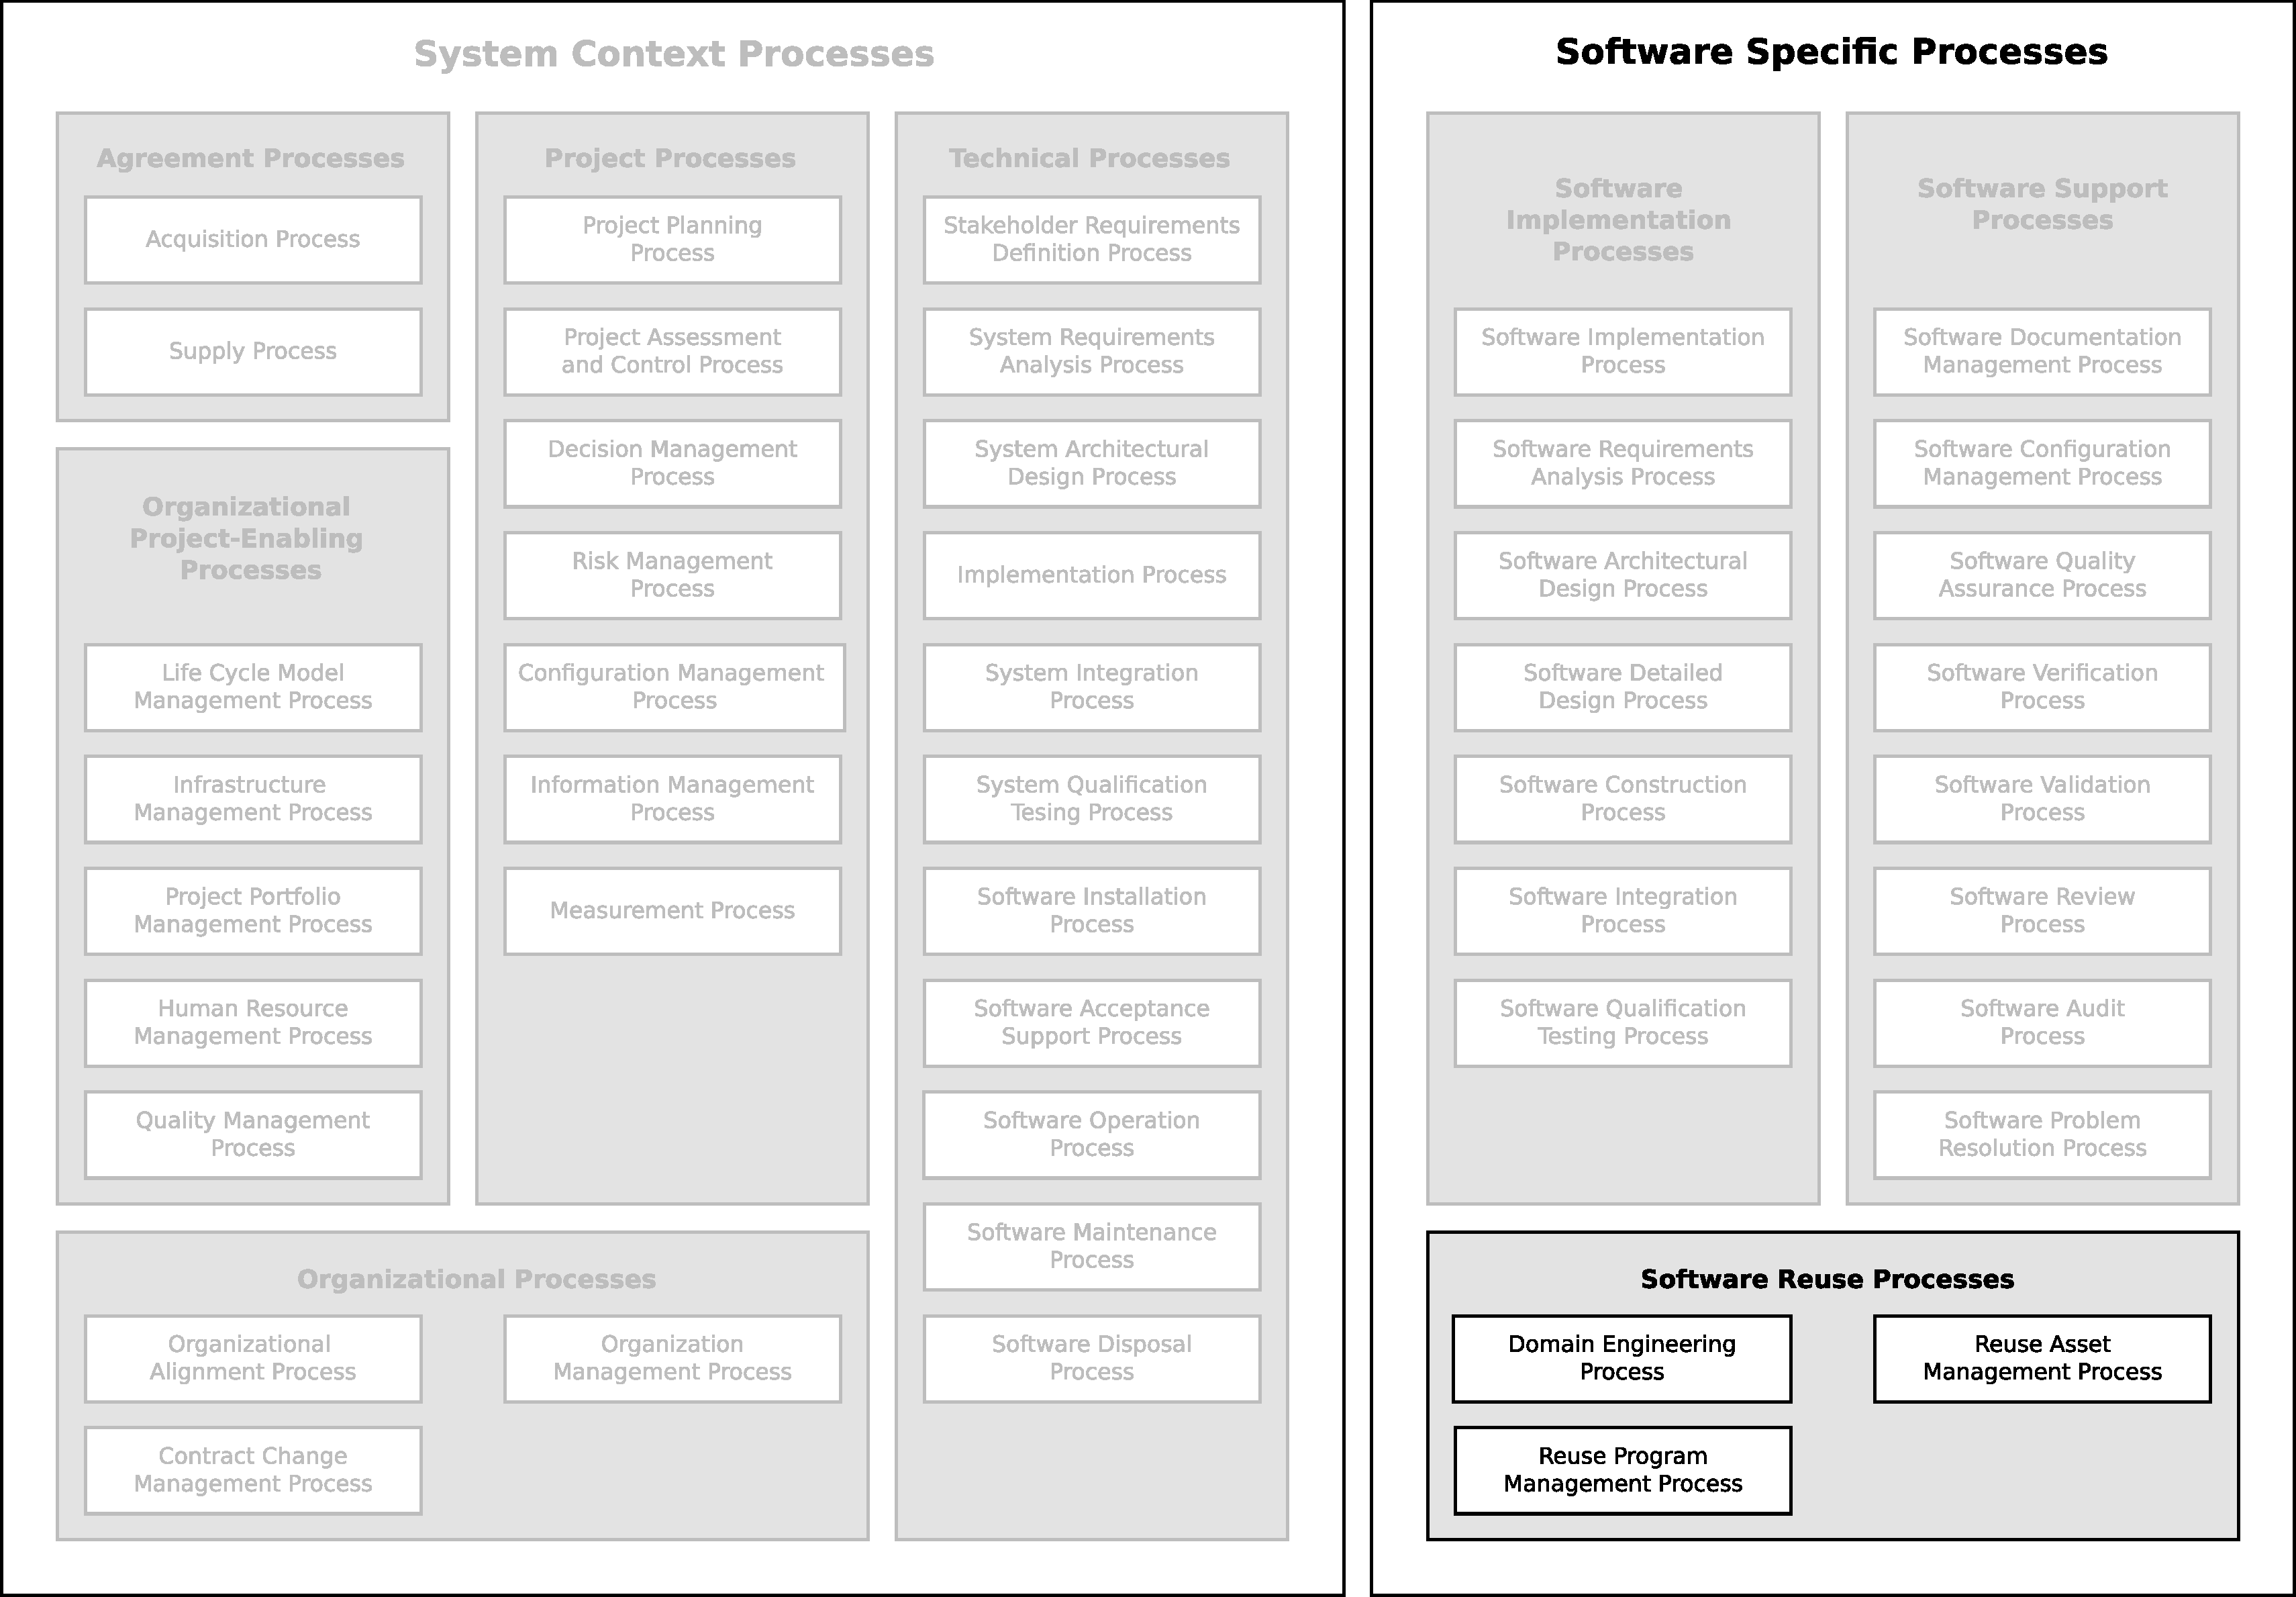
\includegraphics[width=15cm,keepaspectratio]{figures/life-cycle-process-groups-software-reuse-processes.pdf}
			\caption{Software Reuse Processes}
			\label{fig:software_reuse_processes}
		\end{figure}

		\begin{adjustwidth}{1em}{0pt}

			The \nameref{subsec:software_reuse_processes} consist of three processes that support an organization's ability to reuse software items across project boundaries. These processes are unique because, by their nature, they operate outside the bounds of any particular project.

			\begin{compactitem}
				\item \ref{proc:domain_engineering_process} \nameref{proc:domain_engineering_process}
				\item \ref{proc:reuse_asset_management_process} \nameref{proc:reuse_asset_management_process}
				\item \ref{proc:reuse_program_management_process} \nameref{proc:reuse_program_management_process}
			\end{compactitem}

		\end{adjustwidth}

		\newpage
		\subsubsection{DOMAIN ENGINEERING PROCESS\label{proc:domain_engineering_process}}

			\subsubsubsection{PURPOSE}
			\begin{adjustwidth}{2em}{0pt} 

				The purpose of the \nameref{proc:domain_engineering_process} is to develop and maintain domain models, domain architectures and assets for the domain.

			\end{adjustwidth}

			\subsubsubsection{OUTCOMES}
			\begin{adjustwidth}{2em}{0pt} 

				\begin{compactitem}

					\item the representation forms for the domain models and the domain architectures are selected;

					\item the boundaries of the domain and its relationships to other domains are established;

					\item a domain model that captures the essential common and different features, capabilities, concepts, and functions in the domain are developed;

					\item a domain architecture describing the family of systems within the domain, including their commonalities and variabilities, is developed;

					\item assets belonging to the domain are specified;

					\item assets belonging to the domain are acquired or developed and maintained throughout their life cycles; and

					\item the domain models and architectures are maintained throughout their life cycles.

				\end{compactitem}

			\end{adjustwidth}

			\subsubsubsection{ACTIVITIES AND TASKS}
			\begin{adjustwidth}{2em}{0pt} 

				\begin{compactenum}

					\item {\bf Process Implementation}:

					\begin{compactenum}

						\item The domain engineer shall create and execute a domain engineering plan.

						\item The domain engineer shall select the form(s) of representation to be used for domain architectures and models.

						\item The domain engineer shall establish procedures for receiving, resolving, and providing feedback to the asset manager whenever problems or change requests occur for assets developed by the domain engineer.

					\end{compactenum}

					\item {\bf Domain Analysis}:

					\begin{compactenum}

						\item The domain engineer shall define the boundaries of the domain and the relationships between this domain and other domains.

						\item The domain engineer shall identify the current and anticipated needs of stakeholders of software products within this domain.

						\item The domain engineer shall build the domain models using the representation forms selected in the Process Implementation Activity for this process.

						\item The domain engineer shall construct a vocabulary that provides the terminology to describe the important domain concepts and the relationships among similar or common assets of the domain.

						\item The domain engineer shall classify and document the domain models.

						\item The domain engineer shall evaluate the domain models and domain vocabulary in accordance with the provisions of the modeling technique selected and in accordance with the organization’s asset acceptance and certification procedures.

						\item The domain engineer shall conduct domain analysis review(s). Software developers, asset managers, domain experts, and users shall be included in the reviews.

						\item The domain engineer shall submit domain models to the asset manager.

					\end{compactenum}

					\item {\bf Domain Design}:

					\begin{compactenum}

						\item The domain engineer shall create and document the domain architecture, consistent with the domain model and following the organization’s standards.

						\item The domain architecture shall be evaluated in accordance with the provisions of the architecture design technique selected and the organization’s asset acceptance and certification procedures.

						\item For each entity selected to be designed for reuse, the domain engineer shall develop and document an asset specification.

						\item For each asset specified, the specification shall be evaluated in accordance with the organization’s asset acceptance and certification procedures.

						\item The domain engineer shall conduct domain design review(s). Software developers, domain experts, and asset managers shall be included in the reviews.

						\item The domain engineer shall submit the domain architecture to the asset manager.

					\end{compactenum}

					\item {\bf Asset Provision}:

					\begin{compactenum}

						\item The domain engineer shall obtain the asset by acquisition or by development.

						\item The domain engineer shall document and classify the asset.

						\item The domain engineer shall evaluate the asset in accordance with the organization’s asset acceptance and certification procedures.

						\item The domain engineer shall conduct asset review(s). Software developers and asset managers shall be included in the reviews.

						\item The domain engineer shall submit the asset to the asset manager.

					\end{compactenum}

					\item {\bf Asset Maintenance}:

					\begin{compactenum}

						\item When analyzing requests for asset modification and choosing implementation options, the domain engineer shall consider:

						\begin{compactenum}

							\item Conformance with the domain models and the domain architecture;

							\item Impact on the systems and software products that use the asset;

							\item Impact on future users of the asset;

							\item Impact on the reusability of the asset.

						\end{compactenum}

					\end{compactenum}

				\end{compactenum}

			\end{adjustwidth}

		\newpage
		\subsubsection{REUSE ASSET MANAGEMENT PROCESS\label{proc:reuse_asset_management_process}}

			\subsubsubsection{PURPOSE}
			\begin{adjustwidth}{2em}{0pt} 

				The purpose of the \nameref{proc:reuse_asset_management_process} is to manage the life of reusable assets from conception to retirement.

			\end{adjustwidth}

			\subsubsubsection{OUTCOMES}
			\begin{adjustwidth}{2em}{0pt} 

				\begin{compactitem}

					\item an asset management strategy is documented;

					\item an asset classification scheme is established;

					\item criteria for asset acceptance, certification and retirement are defined;

					\item an asset storage and retrieval mechanism is operated;

					\item the use of assets is recorded;

					\item changes to the assets are controlled, and

					\item users of assets are notified of problems detected, modifications made, new versions created and deletion of assets from the storage and retrieval mechanism.

				\end{compactitem}

			\end{adjustwidth}

			\subsubsubsection{ACTIVITIES AND TASKS}
			\begin{adjustwidth}{2em}{0pt} 

				\begin{compactenum}

					\item {\bf Process Implementation}:

					\begin{compactenum}

						\item The asset manager shall create an asset management plan to define the resources and procedures for managing assets.

						\item The asset manager shall execute the plan.

						\item The asset management plan shall be reviewed in accordance with the Software Review Process. Domain engineers and reuse program administrators shall be included in the review.

					\end{compactenum}

					\item {\bf Asset Storage and Retrieval Definition}:

					\begin{compactenum}

						\item The asset manager shall implement and maintain an asset storage and retrieval mechanism.

						\item The asset manager should develop, document, and maintain a classification scheme to be used in classifying the assets.

						\item The asset manager shall conduct review(s) of the asset storage and retrieval mechanism in accordance with the Software Review Process. Reuse program administrators and domain engineers shall be included in the review(s).

					\end{compactenum}

					\item {\bf Asset Management and Control}:

					\begin{compactenum}

						\item For each asset submitted to the asset manager, the asset shall be evaluated based on the asset acceptance and certification criteria.

						\item For each asset accepted, it shall be made available for reuse through the asset storage and retrieval mechanism.

						\item The asset shall be classified in accordance with the reuse classification scheme, if any exists.

						\item The asset manager shall perform configuration management for the asset using the Software Configuration Management Process.

						\item The asset manager shall keep track of each reuse of the asset and report to the domain engineer information about actual reuses of the asset.

						\item The asset manager shall forward asset modification requests and problem reports received from asset reusers to the domain engineer for review and correction/modification plans and actions.

						\item The asset manager shall monitor and record these asset requests/reports and the subsequent actions taken.

						\item The asset manager shall notify all asset reusers, and the domain engineer, of the problems detected in the asset, modifications made to the asset, new versions of the asset, and deletion of the asset from the asset storage and retrieval mechanism.

						\item The asset manager shall retire assets from the asset storage and retrieval mechanism according to the asset retirement procedures and criteria.

					\end{compactenum}

				\end{compactenum}

			\end{adjustwidth}

		\newpage
		\subsubsection{REUSE PROGRAM MANAGEMENT PROCESS\label{proc:reuse_program_management_process}}

			\subsubsubsection{PURPOSE}
			\begin{adjustwidth}{2em}{0pt} 

				The purpose of the \nameref{proc:reuse_program_management_process} is to plan, establish, manage, control, and monitor an organization's reuse program and to systematically exploit reuse opportunities.

			\end{adjustwidth}

			\subsubsubsection{OUTCOMES}
			\begin{adjustwidth}{2em}{0pt} 

				\begin{compactitem}

					\item the organization's reuse strategy, including its purpose, scope, goals and objectives, is defined;

					\item the domains for potential reuse opportunities are identified;

					\item the organization's systematic reuse capability is assessed;

					\item the reuse potential of each domain is assessed;

					\item reuse proposals are evaluated to ensure the reuse product is suitable for the proposed application;

					\item the reuse strategy is implemented in the organization;

					\item feedback, communication, and notification mechanisms that operate between affected parties are established; and

					\item the reuse program is monitored and evaluated.

				\end{compactitem}

			\end{adjustwidth}

			\subsubsubsection{ACTIVITIES AND TASKS}
			\begin{adjustwidth}{2em}{0pt} 

				\begin{compactenum}

					\item {\bf Initiation}:

					\begin{compactenum}

						\item The reuse program for an organization shall be initiated by establishing the organization’s reuse strategy that includes its reuse goals, purposes, objectives, and scope.

						\item A reuse sponsor should be named.

						\item Reuse program participants shall be identified and their roles shall be assigned.

						\item A reuse steering function shall be established to assume the authority and responsibility for the organization’s reuse program.

						\item A reuse program support function shall be established.

					\end{compactenum}

					\item {\bf Domain Identification}:

					\begin{compactenum}

						\item The reuse program administrator, aided by the appropriate manager, domain engineers, users, and software developers, shall identify and document the domains in which to investigate reuse opportunities or in which the organization intends to practice reuse.

						\item The reuse program administrator, aided by the appropriate managers, domain engineers, users, and software developers, shall evaluate the domains to assure that they accurately reflect the organization’s reuse strategy.

						\item The reuse program administrator shall conduct reviews in accordance with the Software Review Process. Software developers, domain engineers, and users shall be included in the reviews.

						\item As more information about the organization’s domains and plans for future software products becomes available or when the domains are analyzed, the domains may be refined and re-scoped by the reuse program administrator.

					\end{compactenum}

					\item {\bf Reuse Assessment}:

					\begin{compactenum}

						\item The reuse program administrator shall assess the organization’s systematic reuse capability.

						\item The reuse program administrator shall assess each domain being considered for reuse to determine the potential for reuse success in the domain.

						\item The reuse program administrator shall make recommendations for refining the organization’s reuse strategy and reuse program implementation plan based on the results of the reuse assessments.

						\item The reuse program administrator, in conjunction with the appropriate acquirers, suppliers, developers, operators, maintainers, asset managers, and domain engineers, shall incrementally improve the skills, technology, reuse processes, organizational structure, and metrics that together comprise the reuse infrastructure.

					\end{compactenum}

					\item {\bf Planning}:

					\begin{compactenum}

						\item A reuse program implementation plan shall be created, documented, and maintained to define the resources and procedures for implementing a reuse program.

						\item The plan shall be reviewed and evaluated for completeness, feasibility of implementation, and ability to realize the organization's reuse strategy. Those evaluating the plan should include members of the reuse steering function.

						\item Approval and support for the reuse program implementation plan shall be obtained from the reuse steering function, and the appropriate managers.

						\item The reuse program administrator shall conduct review(s) in accordance with the Software Review Process. Members of the reuse steering function and the appropriate managers shall be included in the reviews.

					\end{compactenum}

					\item {\bf Execution and Control}:

					\begin{compactenum}

						\item The reuse program administrator shall monitor the progress of the reuse program against the organization’s reuse strategy, and make any necessary adjustments to the plan to realize the strategy.

						\item Problems and non-conformances that occur during the execution of the reuse program implementation plan shall be recorded and resolved.

						\item The reuse program administrator shall periodically reaffirm management sponsorship, support, and commitment to the reuse program.

					\end{compactenum}

					\item {\bf Review and Evaluation}:

					\begin{compactenum}

						\item The reuse program administrator shall periodically assess the reuse program for achievement of the organization’s reuse strategy, and the continued suitability and effectiveness of the reuse program.

						\item The reuse program administrator shall provide assessment results and lessons learned to the reuse steering function, and to the appropriate managers.

						\item The reuse program administrator shall recommend and make changes to the reuse program, expand the reuse program, and improve the reuse program in accordance.

					\end{compactenum}

				\end{compactenum}

			\end{adjustwidth}